
\documentclass[runningheads]{cl2emult}

\usepackage{makeidx}  % allows index generation
\usepackage{graphicx} % standard LaTeX graphics tool
                      % for including eps-figure files
\usepackage{subeqnar} % subnumbers individual equations
                      % within an array
\usepackage{multicol} % used for the two-column index
\usepackage{cropmark} % cropmarks for pages without
                      % pagenumbers
\usepackage{math}     % placeholder for figures
\usepackage{amssymb}     % placeholder for figures
\usepackage{subfigure} % subfigures in one figure

%\usepackage{algorithm2e}
\usepackage[ruled,algonl]{algorithm2e}
%\setlength{\algomargin}{2.1em}
\dontprintsemicolon
\SetInd{0.5em}{1em}
\SetKwFor{Forall}{forall}{do}{od}
\SetKwFor{WhileDo}{while}{do}{od}
\SetKw{Let}{let}

\makeindex            % used for the subject index
                      % please use the style sprmidx.sty with
                      % your makeindex program

%upright Greek letters (example below: upright "mu")
\newcommand{\euler}[1]{{\usefont{U}{eur}{m}{n}#1}}
\newcommand{\eulerbold}[1]{{\usefont{U}{eur}{b}{n}#1}}
\newcommand{\umu}{\mbox{\euler{\char22}}}
\newcommand{\umub}{\mbox{\eulerbold{\char22}}}
\newcommand{\url}[1]{{\small{\tt #1}}}

%%%%%%%%%%%%%%%%%%%%%%%%%%%%%%%%%%%%%%%%%%%%%%%%%%%%%%%%%%%%%

%OPTIONAL%%%%%%%%%%%%%%%%%%%%%%%%%%%%%%%%%%%%%%%%%%%%%%%%%%%%
%
%\usepackage{amstex}   % useful for coding complex math
%\mathindent\parindent % needed in case "Amstex" is used
%
%%%%%%%%%%%%%%%%%%%%%%%%%%%%%%%%%%%%%%%%%%%%%%%%%%%%%%%%%%%%%

%AUTHOR_STYLES_AND_DEFINITIONS%%%%%%%%%%%%%%%%%%%%%%%%%%%%%%%
%
%Please reduce your own definitions and macros to an absolute
%minimum since otherwise the editor will find it rather
%strenuous to compile all individual contributions to a
%single book file
%
%%%%%%%%%%%%%%%%%%%%%%%%%%%%%%%%%%%%%%%%%%%%%%%%%%%%%%%%%%%%%

\begin{document}
%
\title*{The WilmaScope 3D Graph Visualisation System}
%
%
\toctitle{WilmaScope}
% allows explicit linebreak for the table of content
%
%
\titlerunning{WilmaScope}
% allows abbreviation of title, if the full title is too long
% to fit in the running head
%
\author{Tim Dwyer\inst{1}
\and Peter Eckersley\inst{2}
}
%
\authorrunning{Tim Dwyer and Peter Eckersley}
% if there are more than two authors,
% please abbreviate author list for running head
%
%
\institute{School of Information Technologies,
     Madsen Building F09,
     University of Sydney,
     NSW 2006,
     Australia.
		 E-mail: \url{dwyer@cs.usyd.edu.au}
\and Department of Computer Science \& Software Engineering,
     University of Melbourne,
     Victoria 3010,
     Australia.
		 E-mail: \url{pde@cs.mu.oz.au}}

\maketitle              % typesets the title of the contribution



%\begin{abstract}
%The abstract\index{abstract} should summarize the contents of the paper
%in at least 70 and at most 150 words; neither too long
%nor too short but to the point!
%\end{abstract}

\section{Introduction}\label{sec:intro}

\subsection{Witty Survey Subsection}
{\em survey previous stuff.}

\subsection{The Motivation for WilmaScope}
\label{motivation}

Despite, or perhaps because of, the extensive research literature on graph
drawing techniques, there is a lack of state-of-the-art, general-purpose
visualisation systems, particularly for application to 3-dimensional
embeddings.

Graph drawing problems are, of course, existent within an enormous range of
fields; a key motivation for creating a general purpose 3D visualisation
system is to provide easy-to-use components which can be employed by future
software across these application domains.

Within the graph drawing community itself, a system may also aspire to 
streamline, elucidate and beautify the work of algorithm design, comparison
and optimisation.  Achieving these benefits requires software which is
flexible, interactive and easily extensible.

In order to provide these benefits as widely as possible, and to guarantee
an enthusiastic culture of user participation, a serious graph visualisation
system should also be {\em Free Software}\cite{stallman92why}.

In this chapter, we describe WilmaScope (or ``Wilma'', for short), a
sophisticated graph visualisation infrastructure, which attempts to meet
these goals.  In Section~\ref{sec:design}, we describe the Wilma
architecture, modular subsystems, and facilities for control by human users
and other software.  Section~\ref{sec:results} demonstrates Wilma in
action, with examples of graphical results, domain specific applications and
feedback from users.  Finally, Section~\ref{sec:conclusions} reviews Wilma's
contribution and identifies directions for future development.

\section{Design}\label{sec:design}
\subsection{High Level Architecture}
Conceived as a research project with open ended goals, Wilma was
designed to be as flexible and extensible as possible.  The intention
was to allow different components, such as new visual representations
for graph elements, interfaces (either graphical user interfaces or
remote programming interfaces) and different 
layout algorithm implementations to be added or removed easily.
Therefore the design needed to decouple these components as much as
possible so that altering one component would have minimal impact on
the other components.

To achieve this we began by exploring the well known {\em
Model-View-Controller} architecture (MVC) \cite{gamma94design}.
Briefly, the 3 primary components of the MVC architecture are as
follows: 

\begin{description}
\item[Model] the core
of the application, the data and algorithms that automatically modify
the data. 
\item[View] a user interface which displays information
about the model to the user. 
\item[Controller] a separate user
interface that provides methods for the user to manipulate the
application, ie to control the Model.  
\end{description}

Each component's reference to
the other components is via a carefully defined interface which should
not require change when one of the components is modified in some way.  The
standard data flow diagram for the MVC architecture is shown in Figure
\ref{fig-mvc}.

\begin{figure}[h]
  \centering
  \subfigure[MVC Architecture]{
    \label{fig-mvc}
    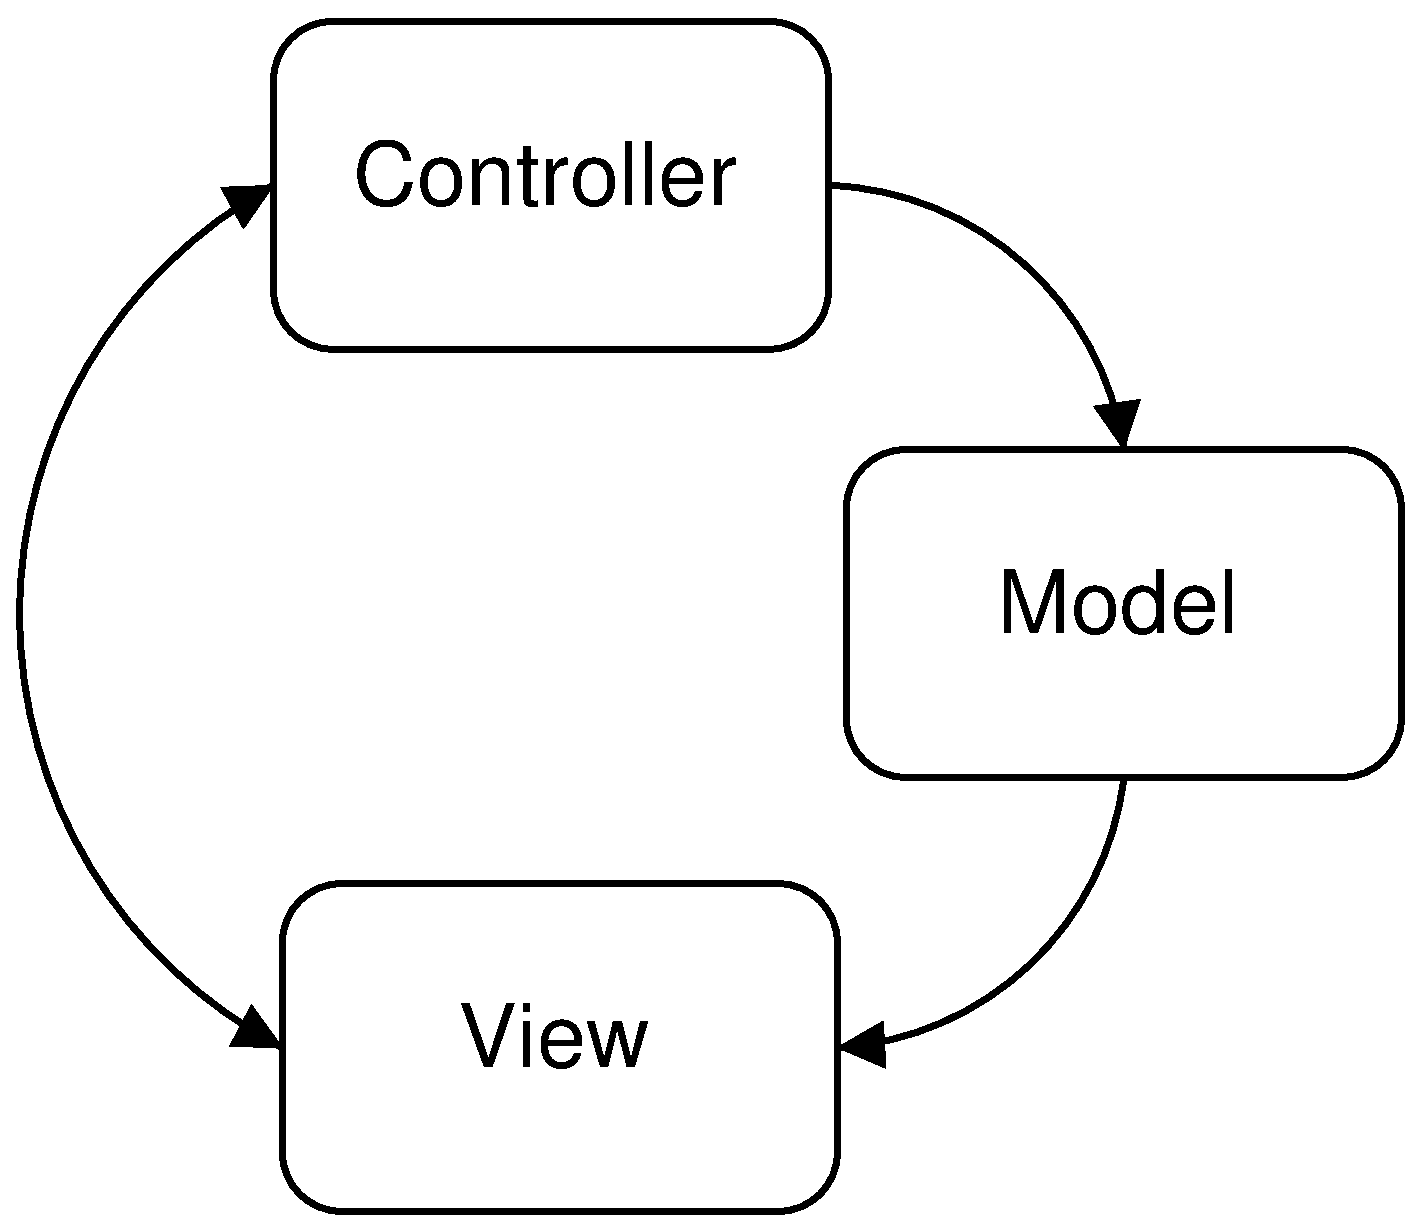
\includegraphics[width=0.4\textwidth]{figures/mvc.eps}}
  \subfigure[Wilma Architecture]{
    \label{fig-wilmamvc}
    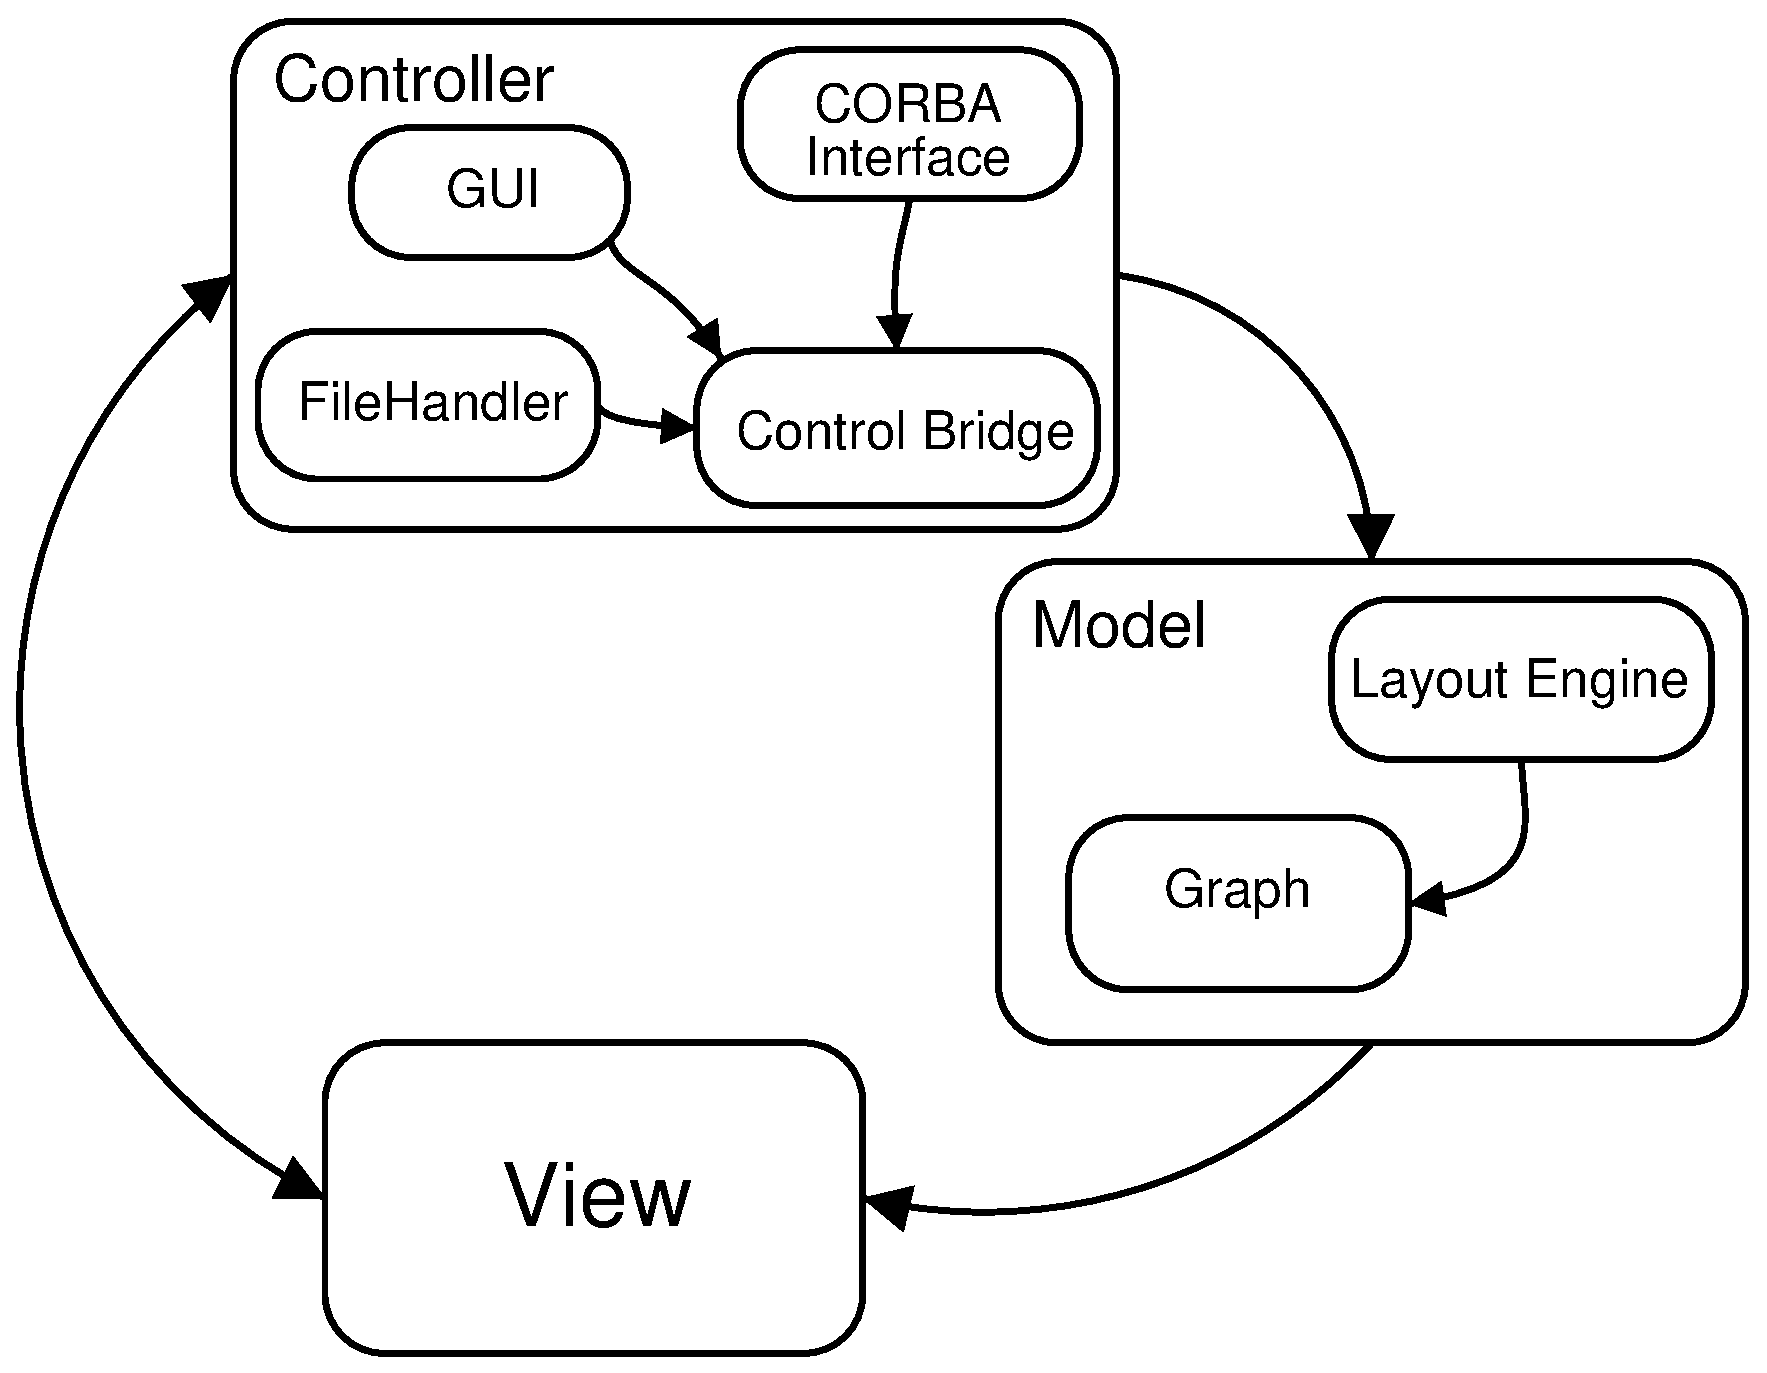
\includegraphics[width=0.5\textwidth]{figures/wilmamvc.eps}}
  \caption{The classic MVC framework and Wilma's utilisation of MVC.}
\end{figure}

In our system the Model component is further broken down into two sub-components:
\begin{description}
\item[Graph] a data structure capable of representing the structure
and state of the graph including its arrangement in space.
\item[Layout Engine] an abstraction of the basic methods required for
an implementation of any layout algorithm that will change the graph's
arrangement in space.
\end{description}

A further requirement for our system is that the graph data model,
the layout engine and the visual representation of the graph elements should be controllable from multiple different sources, primarily:
\begin{description}
\item[Graphical User Interface] a user can interactively construct or edit the graph structure.  Also the user can adjust the layout engine parameters and change the visual representation of the graph elements.
\item[File Handler] a previously constructed graph may be loaded from a file.
\item[API Hooks] supports remote control from a program running in another process or possibly on
another machine. 
\end{description}
The Controller component was therefore also broken
down into several sub-components.  A ``bridge'' layer provides a common
programmatic interface to the Model.  The methods provided by this
bridge layer can then be called by either the GUI interface component,
a component providing a CORBA interface for remote access or a component which
can load and save files to an XML format.

Figure \ref{fig-wilmamvc} depicts this expanded MVC architecture for graph
visualisation. 

\subsection{An Object-Oriented Graph Model}
In designing the Graph Model, ie, the data structures for storing the
graph and the methods for manipulating them, some common
elements were identified.  From the definitions given in Chapter 
\ref{chap-intro}: a graph consists fundamentally
of nodes and edges.  These are the basic graph elements.  A clustered
graph has nodes which may themselves be graphs, or clusters.

This description of a graph is modelled in a class hierarchy by
defining an abstract class {\em GraphElement} which is implemented by
both the {\em Node} and {\em Edge} classes.  A {Cluster} will inherit
all the properties of the {\em Node} class and also contains an
aggregation of {\em Nodes} and {\em Edges}.  A {Cluster} also contains
a reference to an abstract definition of a {\em LayoutEngine} which
provides a common interface to an implementation of a layout algorithm
for arranging the graph in 2 or 3 dimensional space.  Since the
details of the algorithm are kept separate it is easy to mix and match
different layout styles to different graphs or even clusters within
the one graph.  A similar class hierarchy was developed independently
by Marshall et.  al\cite{marshall00object} around the same time.
Figure \ref{fig-wilmaclasses} shows a UML diagram depicting this
graph class hierarchy, and also shows how this relates to a force
directed {\em LayoutEngine} implementation, discussed further in
Section \ref{sec:forcedirectedlayout}.  In Figure
\ref{fig-wilmaclasses3d} we show a 3D
interpretation of this UML diagram rendered by Wilma in an application
of the system described further in \ref{sec:3duml}.

\begin{figure}[h]
  \centering
  \subfigure[UML Class diagram.]{
    \label{fig-wilmaclasses}
    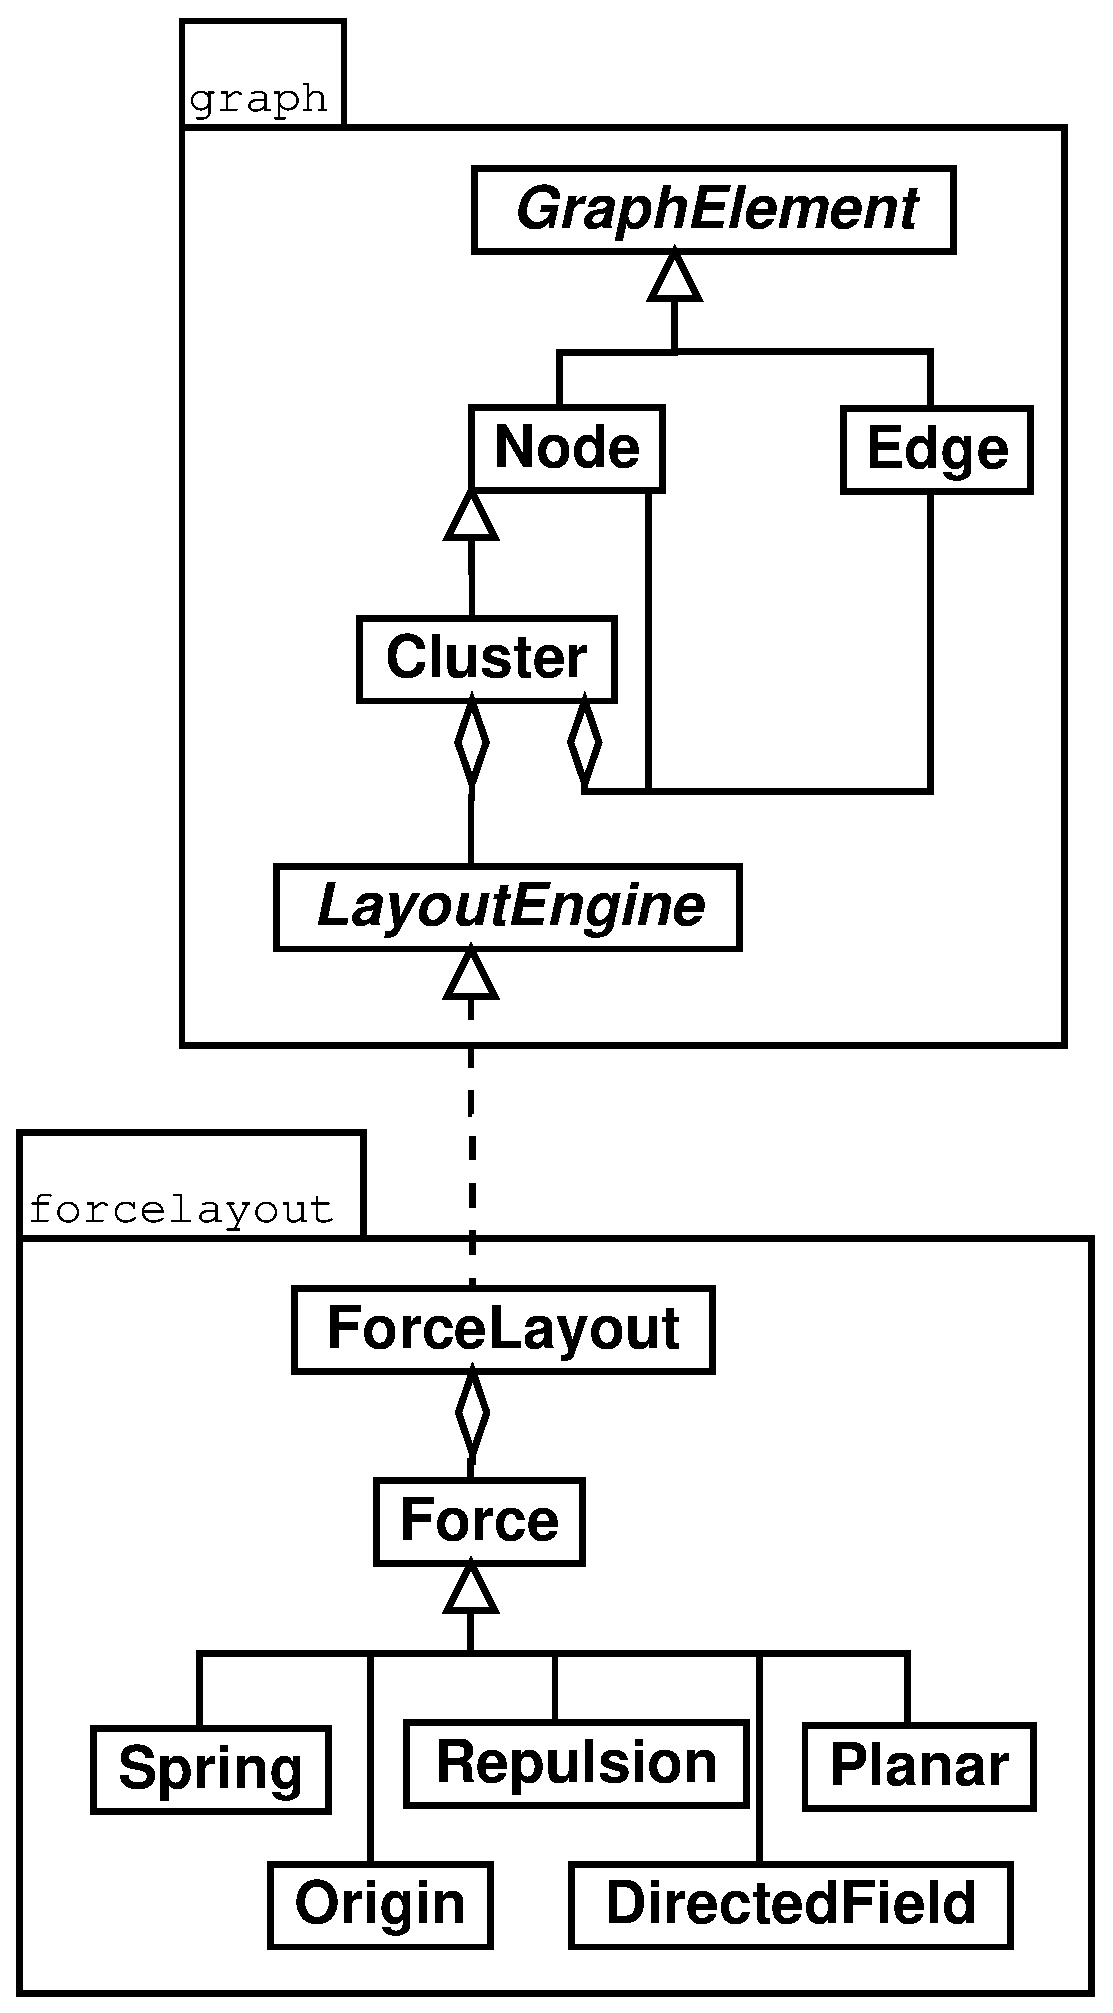
\includegraphics[width=0.35\textwidth]{figures/wilmaclasses.eps}}
  \subfigure[A 3D interpretation of the class hierarchy.]{
    \label{fig-wilmaclasses3D}
    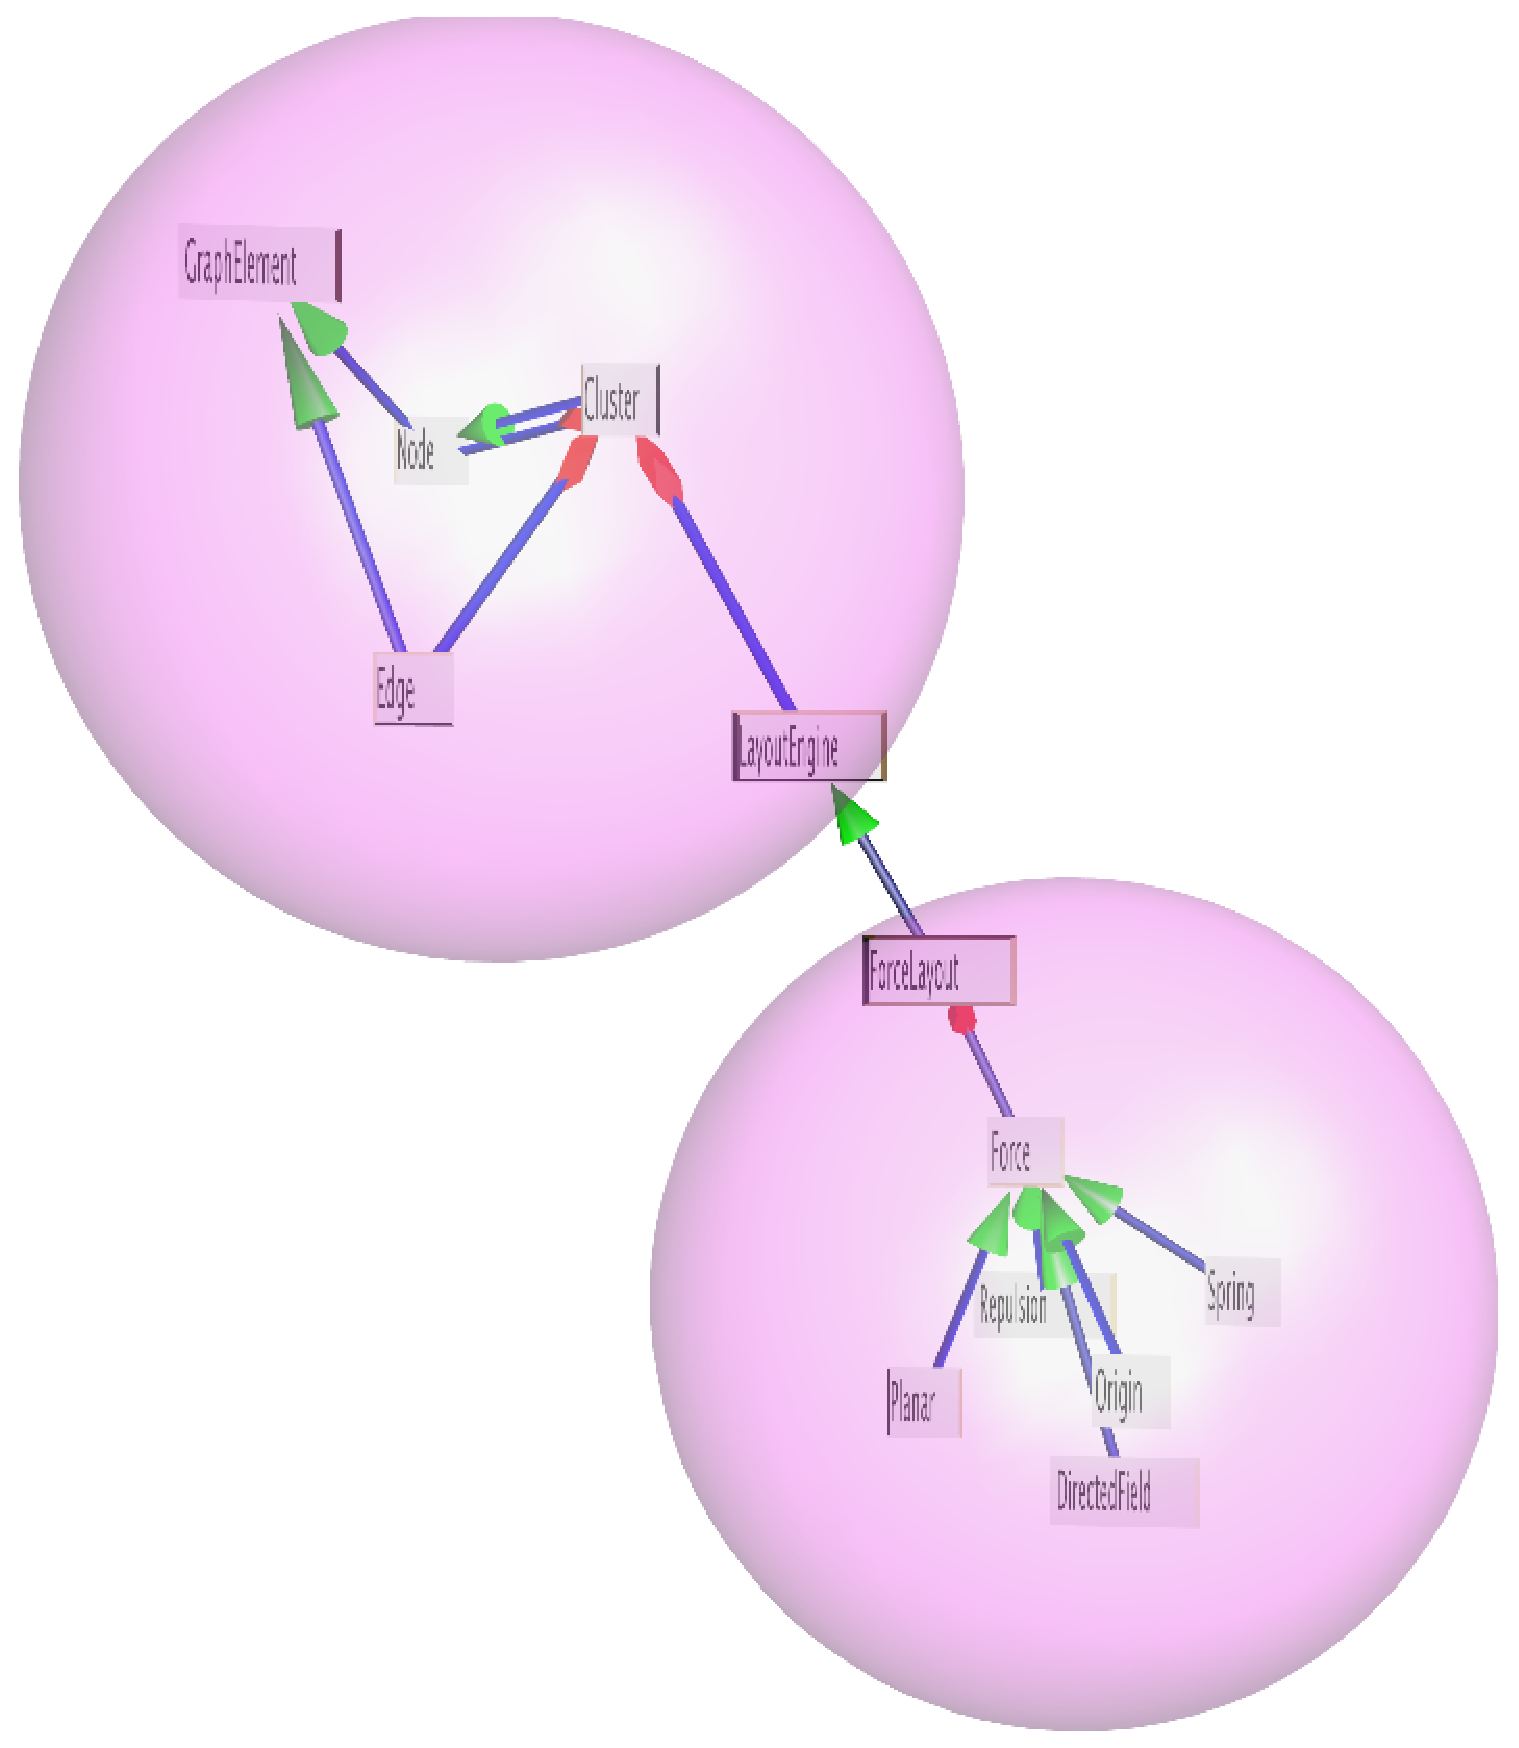
\includegraphics[width=0.55\textwidth]{figures/wilmaclasses3d.eps}}
  \caption{A class hierarchy for the graph model and the classes used
  in the Force Directed Layout Engine implementation.}
\end{figure}

\subsection{User Interface Design}
A screenshot of the main Wilma window, with labels describing the main
features is shown in Figure \ref{fig-controls}.
The majority of the space in this window is given over to the 3D
canvas in which the graph structure is visualised.  Users may ``fly''
through the virtual space rendered on this canvas by dragging with the
various mouse buttons.  The possible mouse navigation actions (rotate,
zoom and translate) are
shown in the reminder panel at the bottom of the window.

The user may also navigate through the cluster hierarchy through this
window.  Clusters are generally shown as transparent spheres or other 

Wilma was conceived as an interactive graph editor and therefore there
are a range of basic actions which a user may perform in editing the
graph structure.
\begin{figure}[h]
  \centering
    \label{fig-controls}
    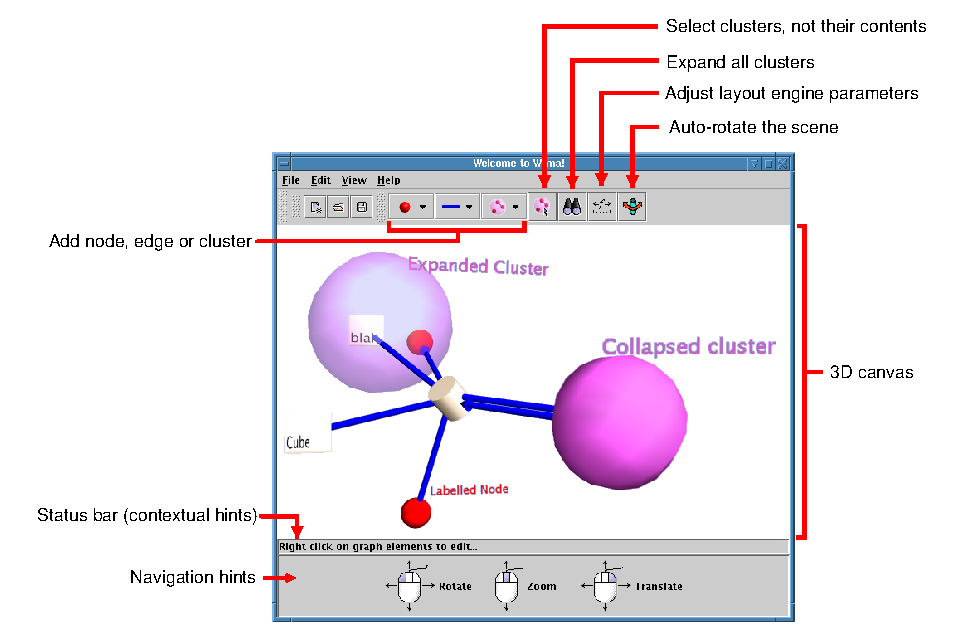
\includegraphics[width=0.7\textwidth]{figures/wilmacontrols.eps}
\end{figure}

\begin{figure}
  %\subfigure[Controls for generating random graphs for testing layout
  %algorithms]{
    %\label{fig-randomcontrols}
%\scalebox{0.3}{
%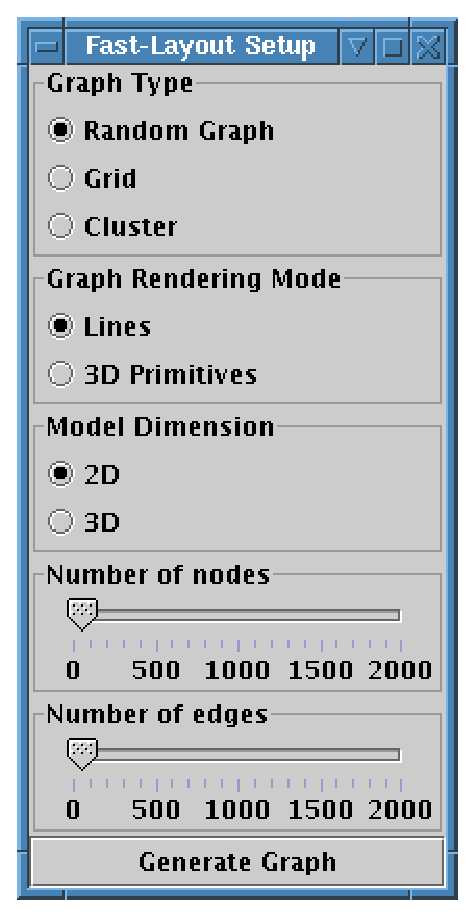
\includegraphics{figures/wilma-randomcontrols.eps}}}
  \subfigure[Controls for the force directed layout engine]{
    \label{fig-forcecontrols}
\scalebox{0.3}{
    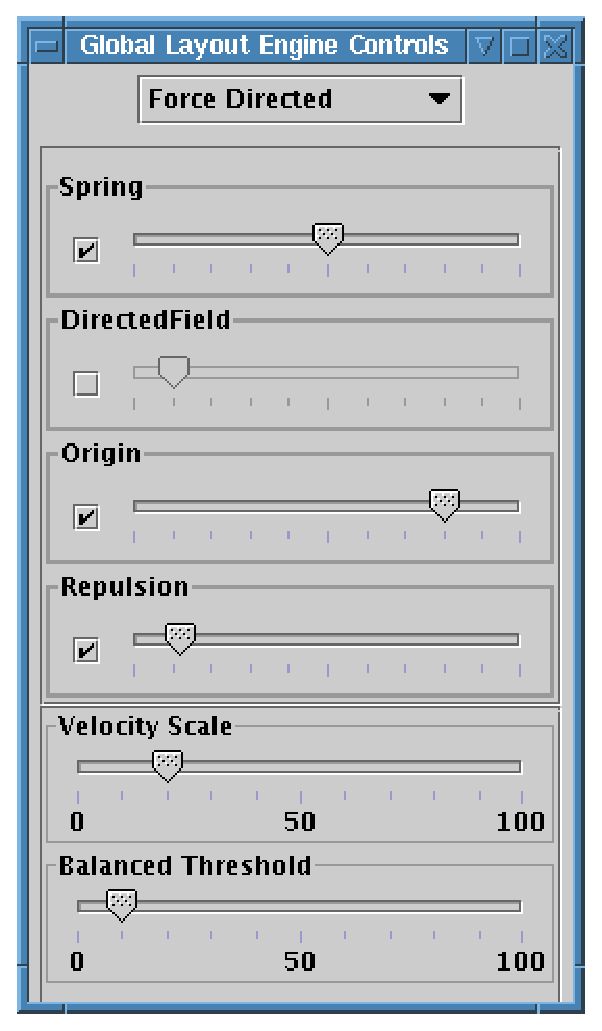
\includegraphics{figures/wilma-forcecontrols.eps}}}
  \subfigure[Controls for the multiscale force directed layout
  engine]{
    \label{fig-multiscalecontrols}
\scalebox{0.3}{
    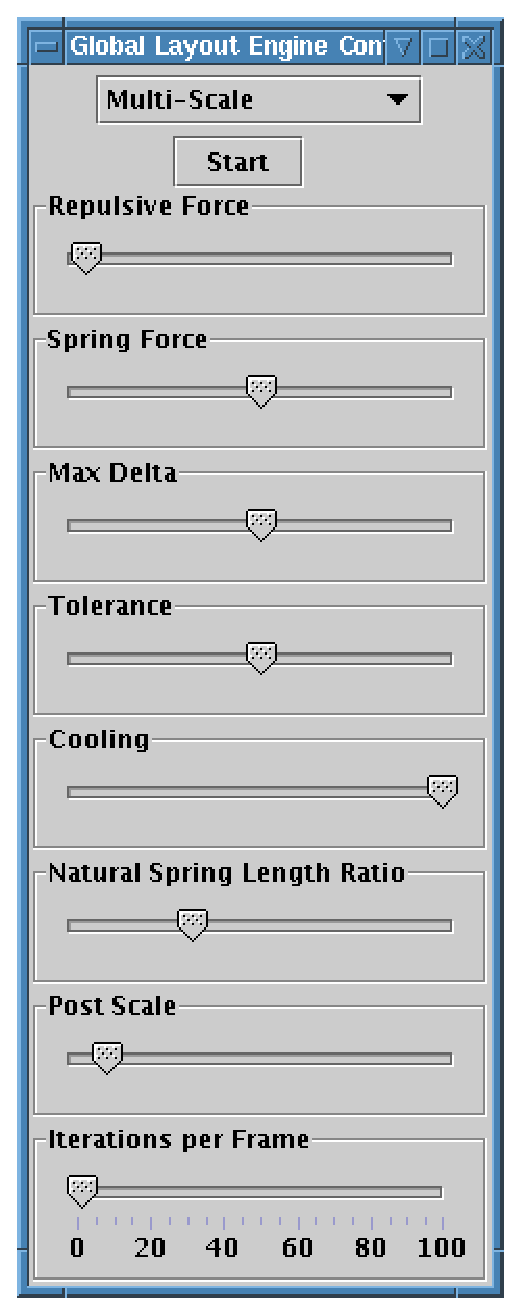
\includegraphics{figures/wilma-multiscalecontrols.eps}}}
  \subfigure[Controls for the simulated annealing layout engine]{
    \label{fig-simannealcontrols}
\scalebox{0.3}{
    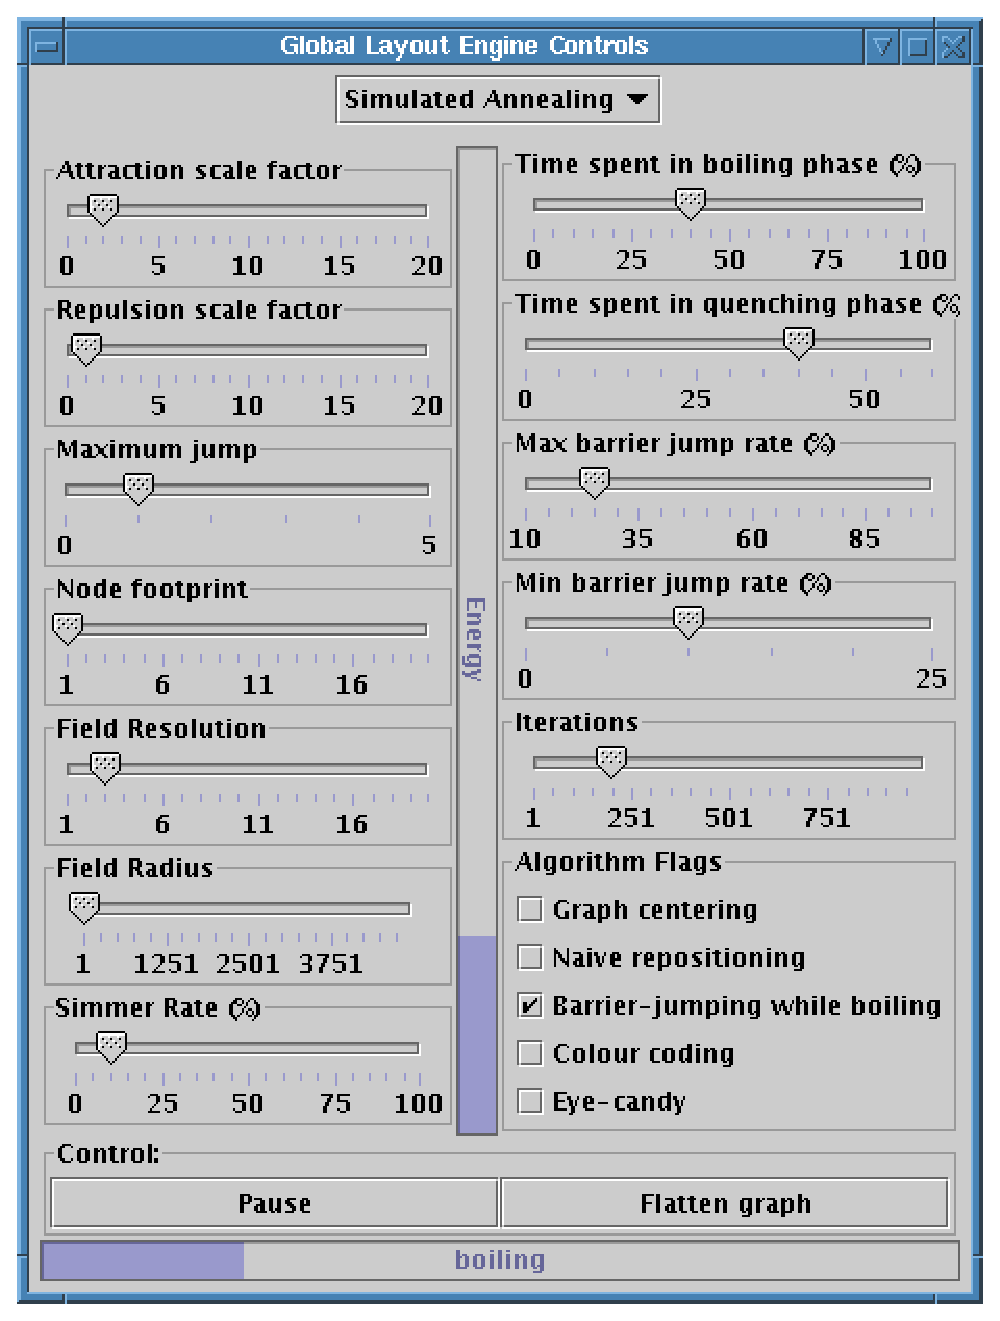
\includegraphics{figures/wilma-simannealcontrols.eps}}}
  \caption{The various layout engine control windows in Wilma.}
\end{figure}

\subsection{Platform}

WilmaScope has been implemented in Java, using the Java3D graphics library.
Java provides a good tradeoff between high level language constructs,
portability and performance.  Java3D provides access to 3D graphics accelerator hardware through
a high-level Java API and useful features such as a scene graph
structure and methods for coupling animation into the render cycle.

\subsection{Layout Algorithms}
\subsubsection{Force Directed} \label{sec:forcedirectedlayout}
The first layout algorithm implemented in Wilma was Force Directed
layout whose basic principles are described in Chapter
\ref{chap-intro}.  There were several factors that led us to
implement this algorithm first, notably:
\begin{itemize}
\item it is relatively easy to obtain good results for most types of
graphs by application of the basic attractive spring force and
repulsive inter-node force.
\item it is easy to animate the layout process in a dynamic
graph visualization to preserve a user's ``mental map''\cite{Misue:VLC95}
between changes in the graph structure.  We can animate simply by
redrawing the graph between each iteration of the algorithm.
\item since the algorithm is iterative and does not require any
special pre or post-processing it is easy to use in a dynamic graph
editor, where the graph structure may be changed by the user even
before the layout has stabilised.
\item different layout
aesthetics can be enhanced by adding extra forces, such as the Sugiyama and Misue\cite{Sugiyama:VLC95}
directed field force for aligning directed edges to emphasise flow.
\item the force directed approach can be easily extended to support
clustered graphs \cite{Huang:GD98}
\item it works just as well in 3-dimensions as in 2.
\end{itemize}
The wilma implementation of the force directed algorithm attempts to make the most
of all of these advantages.  Firstly it offers a user interface which
allows the user to control all the parameters of the layout algorithm
even while the layout is still in progress.  The user can control the
number of iterations of the algorithm that are executed between frames
of animation so that they can choose to run the algorithm to
convergence as fast as possible or to watch the layout unfold, and if
necessary tweak the controls to adjust the layout or to help it
converge.

Different forces, such as the directed field force or
a gravitational force which keeps the graph centred, may be added or removed
at any time to achieve different aesthetic effects.  Figure
\ref{fig-wilmaclasses} gives the UML class diagram for the force
directed layout engine.  Since each of the different forces implements
a common interface new forces can be added or removed at any time.

Finally the force directed layout engine fits well into Wilma's object
oriented clustered graph model.  As mentioned previously each cluster
has its own layout engine but when the force directed engine is used,
edges connecting nodes in different clusters exert a force on
the nodes inside these clusters.  The nodes inside a cluster are
attracted to the centroid of the cluster by a ``gravitational force''.
The gravitational force then balances the inter-cluster forces.  This
achieves a net result similar to the ``dummy node'' approach of Huang
and Eades\cite{Huang:GD98} however repulsive forces do not need to be
calculated between nodes inside different clusters.

A novel extension that has been added to our force directed layout
engine is the ability for the contents of clusters to be constrained
to a plane.  The orientation of this plane is then able to rotate in
order to help minimise the spring force of inter cluster edges.  This
is illustrated in Figure \ref{fig-spincluster}.  By restricting the
contents of clusters to planes, but then allowing the clusters
themselves to be arranged in 3-Dimensions allows certain types of
clustered
graphs to be more clearly displayed.  For example a graph which is not
c-planar\cite{Eades:GD96} but which has planar clusters may be best
shown in this way to show planarity where possible but to avoid
intersecting edges.
\begin{figure}[h]
  \centering
    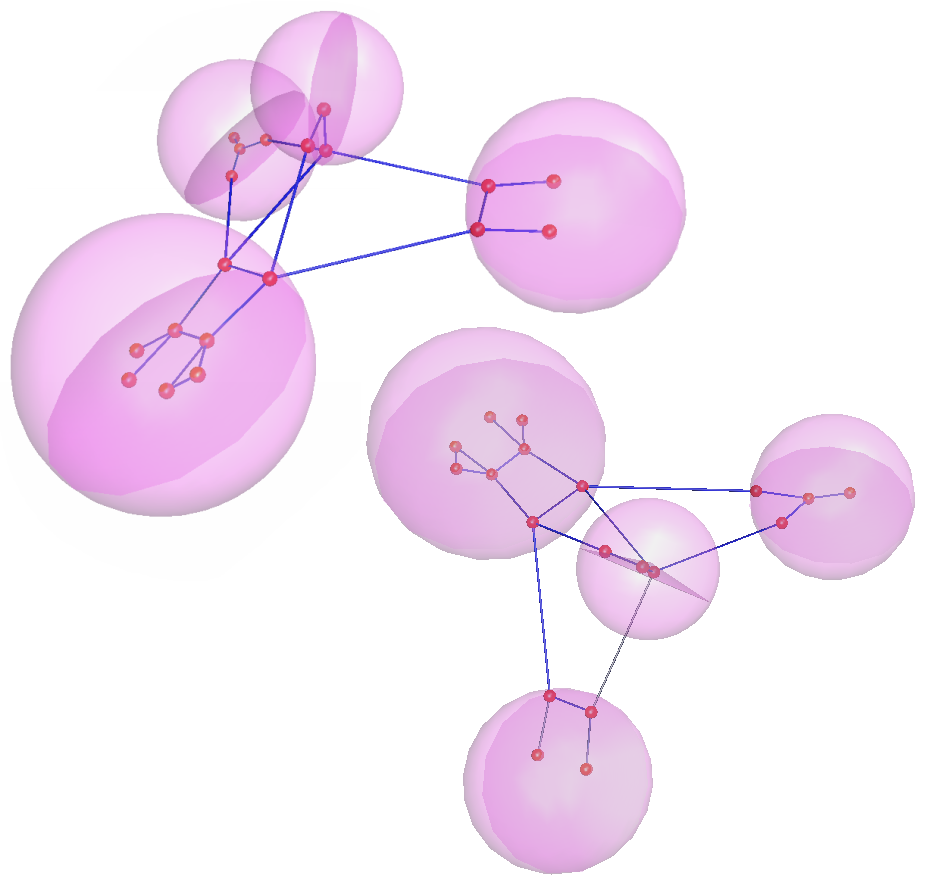
\includegraphics[width=0.8\textwidth]{figures/enterprise.eps}
  \caption{A screenshot showing a clustered graph with planar
  clusters.  The clusters are rotated to minimise the lengths of the
  edges between clusters.}
  \label{fig-spincluster}
\end{figure}

\subsubsection{Fast Simulated Annealing}

As we stated in Section~\ref{motivation}, a major design goal for Wilma
was to provide a platform within which algorithmic experimentation could be
conducted elegantly and efficiently.

Force-directed layout algorithms are of course the method of choice for a
wide range of graph visualisation problems.  One variation on these
algorithms, advocated by Fruchtermann \&
Rheingold~\cite{fruchtermann90force-directed} and Davidson {\em et.
al.}~\cite{davidson01noise}, attempts to avoid calculation of repulsion force
vectors, which is $O(n)$ in the number of vertices for each node $i$, and
$O(n^2)$ for the whole graph:

\begin{equation}
\label{repulsion}
\vec{R}_i \equiv \sum_{j \in V \setminus \{i\}} \vec{r}_{i,j}
\end{equation}

\noindent Where $\vec{r}_{i,j} = \vec{r}_i - \vec{r}_j$ is the displacement
of node $i$ relative to $j$.

To avoid this expense, it is possible to approximate scalar energy potential
values, caching this information at grid points throughout space.  Iterated
updates to the potential well then cost only $O(|V|)$ time per iteration.  On
the downside, the cache array itself takes $O(v \centerdot \rho)$ memory,
where $v$ is the $n$-dimensional volume (or area) of the embedded graph and
$\rho$ is the density of stored potential data points.

Cowling~\cite{cowling02fast} has implemented a fast layout engine for
WilmaScope which employs simulated annealing with potential energy caching to
achieve linear-time graph embeddings.  Cowling was able to demonstrate that
the algorithms of \cite{davidson01noise} do appear to achieve linear time
results, but that when the grid size $v \centerdot \rho$ must be adjusted to
prevent folding in large graphs, space and time complexity are no longer
linear.  Figure \ref{fig-fastlayout} shows before and after screenshots of
the algorithm's effects.

Cowling's work serves to demonstrate the utility of Wilma as an empirical
platform; with the WilmaScope rendering and navigation system, and the
availability of convenient data structures for input and dataset management,
algorithmic experiments can be performed at optimal speeds.

\begin{figure}[h]
  \centering
  \subfigure[After only a few iterations.]{
    \label{fig-fastlayout1}
    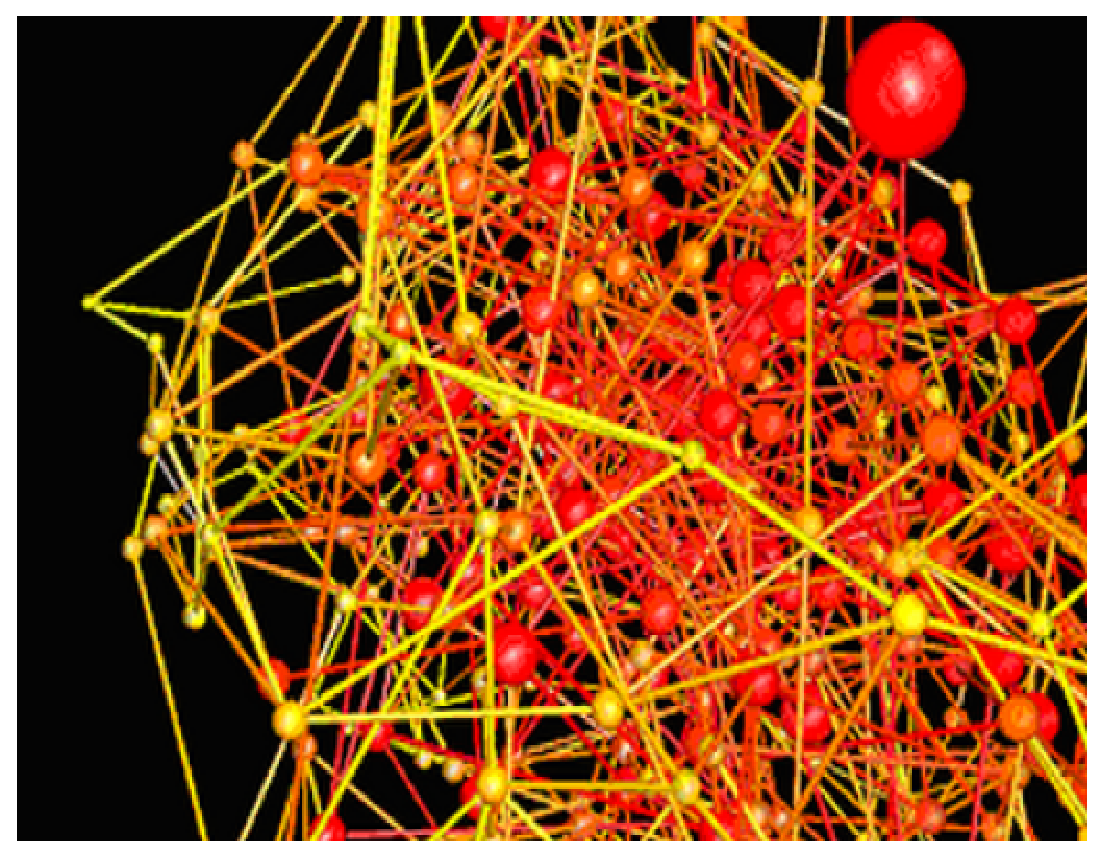
\includegraphics[width=0.4\textwidth]{figures/fastlayout1.eps}}
  \subfigure[After a complete run of the algorithm.]{
    \label{fig-fastlayout2}
    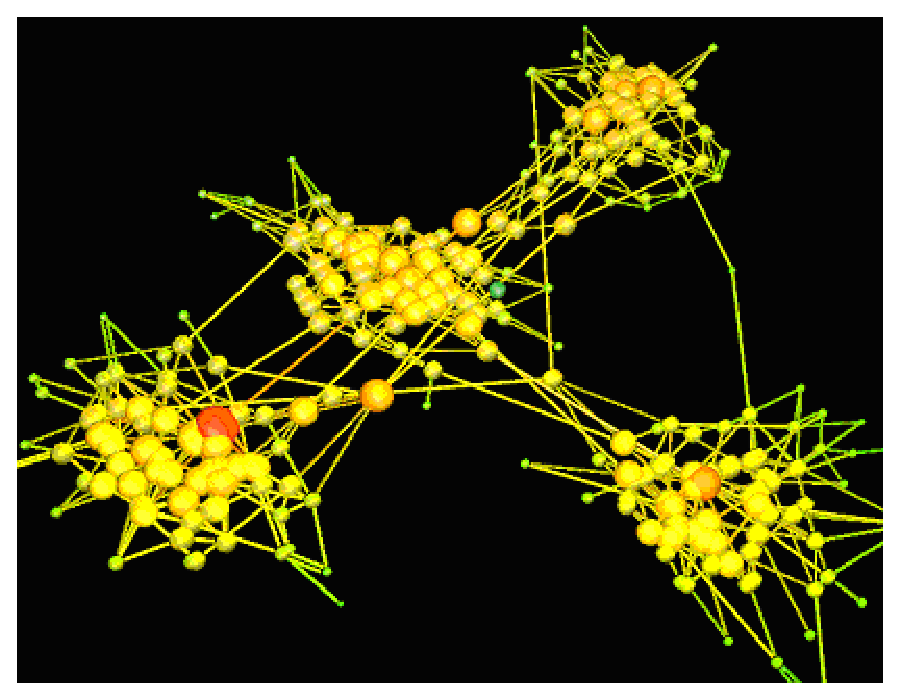
\includegraphics[width=0.4\textwidth]{figures/fastlayout2.eps}}
  \caption{These screenshots demonstrate the effects of the simulated
  annealing algorithm with potential caching.  Note that the colour of
  the nodes indicates the force potential at that location.}
  \label{fig-fastlayout}
\end{figure}


\subsubsection{Multiscale Force Directed}

Although the fast simulated annealing approach described above did not prove
perfect as a universal replacement for iterated, force-directed layout, there
are other algorithms in the literature which might be brought to bear.

We have implemented one of these - the ``Multilevel Force-Directed'' approach
of Walshaw~\cite{walshaw00multilevel}.  This multi-scaled approach
incorporates two main innovations over the common or garden force-directed
algorithm -- hierarchical layout, and short-range-only repulsion forces.

Instead of laying out the entire graph from singular or random initial
conditions, the algorithm creates a series of simplified approximations of
the graph, and embeds each of these with increasingly fine detail.

The simplified approximations are generated by applying matching algorithms,
which, at each iteration, select as many edges as possible such that
no node is connected to two of these edges.  Each edge is then ``collapsed''
so that the two nodes at either end are combined, and the process is repeated.

In order to perform these simplifications rapidly, the stochastic matching
approach of Hendrickson \& Leland~\cite{hendrickson95multilevel} is employed,
which takes $O(|V| \centerdot {|E| \over |V|})$ time, and is linear for
sparse graphs.

After each level of force-directed layout has stabilised, the aggregated
nodes are replaced by their pairs of matched children, and the thermal energy
of the system is re-initialised.  This process repeats until the entire graph
has been embedded.

The multilevel process provides a number of benefits over single-pass force
directed layout.  Notably, these include avoidance of local energy minima
which may result from the arbitrary initial position of a large set of nodes;
and the ability to tune layout parameters to correct for pathologies which
become apparent to the user, as the level of detail increases.

Walshaw's algorithm also addresses the $O(n^2)$ cost of the calculating the
repulsion force (see Equation~\ref{repulsion}).  As with the fast simulated
annealing strategy, this involves storing information about the repulsion in
a spatial data structure, although the details are different.

Instead of trying to approximate the potential field of the force, the
spatial structure simply allows nodes to be addressed by their locality (or
``cell'').  A na\"{i}ve method of doing this is to keep lists of nodes in a
complete spatial array.  The size of an array may become large relative to
the number of nodes (especially for spacious 3D embeddings), but if this is
problematic, then space usage can be made linear in the number of nodes in
exchange for a constant slowdown, through the use of a hash table.

If the repulsion force is constructed so that it cuts off beyond a certain
distance $d_\infty$, that is:

\begin{equation}
\exists \, d_\infty : \, 
||\vec{r_i} - \vec{r_j}|| > d_\infty
\Rightarrow 
repulsionforce (\vec{r_i},\vec{r_j}) = \vec{0}
\end{equation}
%\forall d > d_\infty, f_g(d) = 0

Then it is possible to calculate the repulsion force on a particular node $i$
with reference solely to the positions of nearby nodes.  If the cells for
the spatial data structure are of a size greater than or equal to $d_\infty$,
then all such nodes may be addressed through the cell containing $i$, and
those adjacent to it.  In this algorithm, the cost of calculating the
replusion force is $O(|V| \centerdot \rho)$, where $\rho$ is the average 
of the embedding density around each node.  Provided that the repulsion
force is {\em strong} --- that it does not fall of faster than the square
of the distance between nodes --- then we can expect $\rho$ to be bounded
independently of $|V|$, and thus, repulsion force evaluation to be linear.

The multilevel force-directed layout engine thus provides WilmaScope with
an efficient mechanism for handling large graphs.

\subsubsection{DOT: heirarchical layout}
DOT is a program included in the Graphviz
(\url{http://www.graphviz.org}) open source graph visualisation
toolkit from AT\&T.  It produces effective 2-dimensional layered graph
layouts using a Sugiyama\cite{Sugiyama81methods} style algorithm.
The Wilma DOT layout engine runs dot in a sub-process, pipes in the graph
data converted into DOT file format and parses the DOT output to
obtain the new layout.
DOT also features aesthetically pleasing spline edges which Wilma
is able to render as curved tubes.

Since the DOT layouts are strictly 2-dimensional we are free to use the
third dimension to capture additional information.  For example
Section \ref{sec:fmflow} describes an application where the 3rd
dimension (the {\em z}-axis) is used to capture changes in the graph over time.
That is, the nodes are rendered as tubes and the edges may appear at different
levels in the {\em z} dimension.

\subsection{User Interfaces}
\subsection{Programming Interfaces}
\label{API}

A key design goal for Wilma was the provision of graph visualisation
facilities for other programs with very low barriers to development.  In order
to achieve this, we have implemented two external access APIs which give
programmers the ability to call up, extend and manipulate graph visualisations
in real-time.  These are the WilmaChat graph definition language, and the
Wilma CORBA interface.

\subsubsection{WilmaChat: A Dialogue on Graph Structure}

The simplest and lowest-energy programming interface to Wilma is the WilmaChat
language.  WilmaChat operates by invoking a server daemon which listens on a
socket or pipe on the machine in question.

Clients can connect to WilmaChat and control graphs by passing commands
in a simple language which allows them to instantiate arbitrary graph
structures.

The advantage of WilmaChat is that it requires extremely little infrastructure
from the developer's programming environment.  The ability to traverse
internal graph structures and print a simple, formalised description of them
is enough to produce navigable 3D output.

\subsubsection{The Wilma CORBA Interface}

While the WilmaChat language is extremely efficient for rapid application
development, and can be driven by any programming environment on Wilma's
supported platforms, there are a number of advanced features for which the
socket dialogue is an inefficient mode of interaction.  For example, if
developers want multiple clients to connect to a particular Wilma server, in
the presence of access-control mediation; or if they wish to perform detailed
interrogation of the graph embedding which Wilma has created --- then the use
of a custom language requires more overhead.

In order to meet these more sophisticated requirements, we have implemented a
Wilma control interface which sits atop CORBA (the Common Object Request
Broker Archicture --- see \url{http://www.corba.org}).  Since CORBA provides
its own access control mechanisms, and good CORBA bindings handle all the
marshaling and type requirements for a sophisticated API, programmers using
languages which support CORBA can take advantage of these facilities without
writing additional code.

\section{Results: The Importance of being Wilma}
\label{sec:results}
Wilma was designed to be as open and extensible as possible and
evidence for the success of this design is shown in the array of
domains to which Wilma has been applied.

\subsection{Applications}
\subsubsection{3D UML Visualisation} \label{sec:3duml}
The first application of Wilma was an investigation into a 3D
extension of the Unified Modelling Language\cite{dwyer013D-UML}.
UML diagram elements were translated into 3D glyphs and a simple class
diagram editor was constructed on top of the Wilma framework.  A user study
was then conducted to test the feasibility of such a paradigm for
software design.  Interesting annecdotal evidence was collected
indicating that such 3D UML models, when coupled with a force directed
layout engine could help a software architect to understand structure
within a reasonably complex system.  An example of such a diagram is
shown in Figure \ref{fig-wilmaclasses3D}.

\subsubsection{Fund Manager Flow Visualisation} \label{sec:fmflow}
Most stock market visualisations involve a fairly straightforward
mapping of share attributes into 2 or 3 dimensional space.  The most
obvious example is share price time series charts.  In an experiment
into graph based visualisation techniques for stock market data
Dwyer~\cite{dwyer02fmflow} defined a graph model for Fund Manager
movement within the stock market.  The graph consists of nodes
representing stocks and edges representing a {\em movement} of a
fund manager between a pair of stocks.  A movement from one stock to
another occurs when a fund manager reduces his holding in the first
and increases his holding in the second.

The clients were particularly interested in seeing the changing
behaviour of fund managers over time.  This turned out to be a problem
of visualising a changing graph.  We showed these changes by
arranging the graph for each time period on a plane and then stacking
the time periods in the third dimension.  Nodes representing stocks
are extruded into columns whose width may be varied to indicate a
stock attribute such as unit price.  We call these 3D stacked graph
visualisations {\em stratified graphs}, borrowing the geological term.

Various styles of layout were tried in arranging these stratified
graphs in space.  Force
directed layout was useful for showing clustering and centrality of
highly active stocks while sugiyama style layout is useful for showing
flow from source stocks to sinks.  Figure \ref{fig-fm} shows an
example using the DOT layout engine in Wilma to produce 3D sugiyama
style layout.  A current research project is to tailor the hueristics
used in these layout algorithms to suit such stratified graphs.

\begin{figure}[h]
  \centering
  \subfigure[]{
    \label{fig-fmflow}
    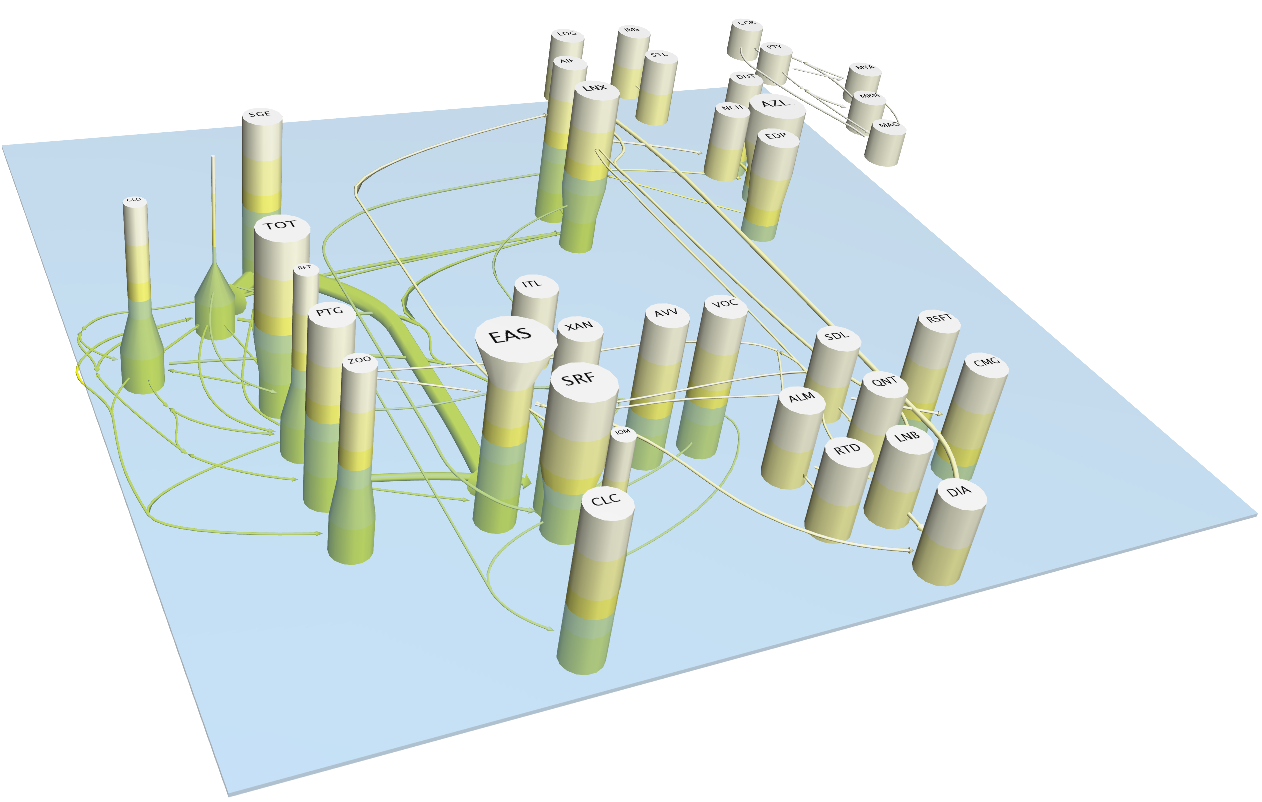
\includegraphics[width=0.5\textwidth]{figures/dot_waterlevel2.eps}}
  \subfigure[Side view]{
    \label{fig-fmflow}
    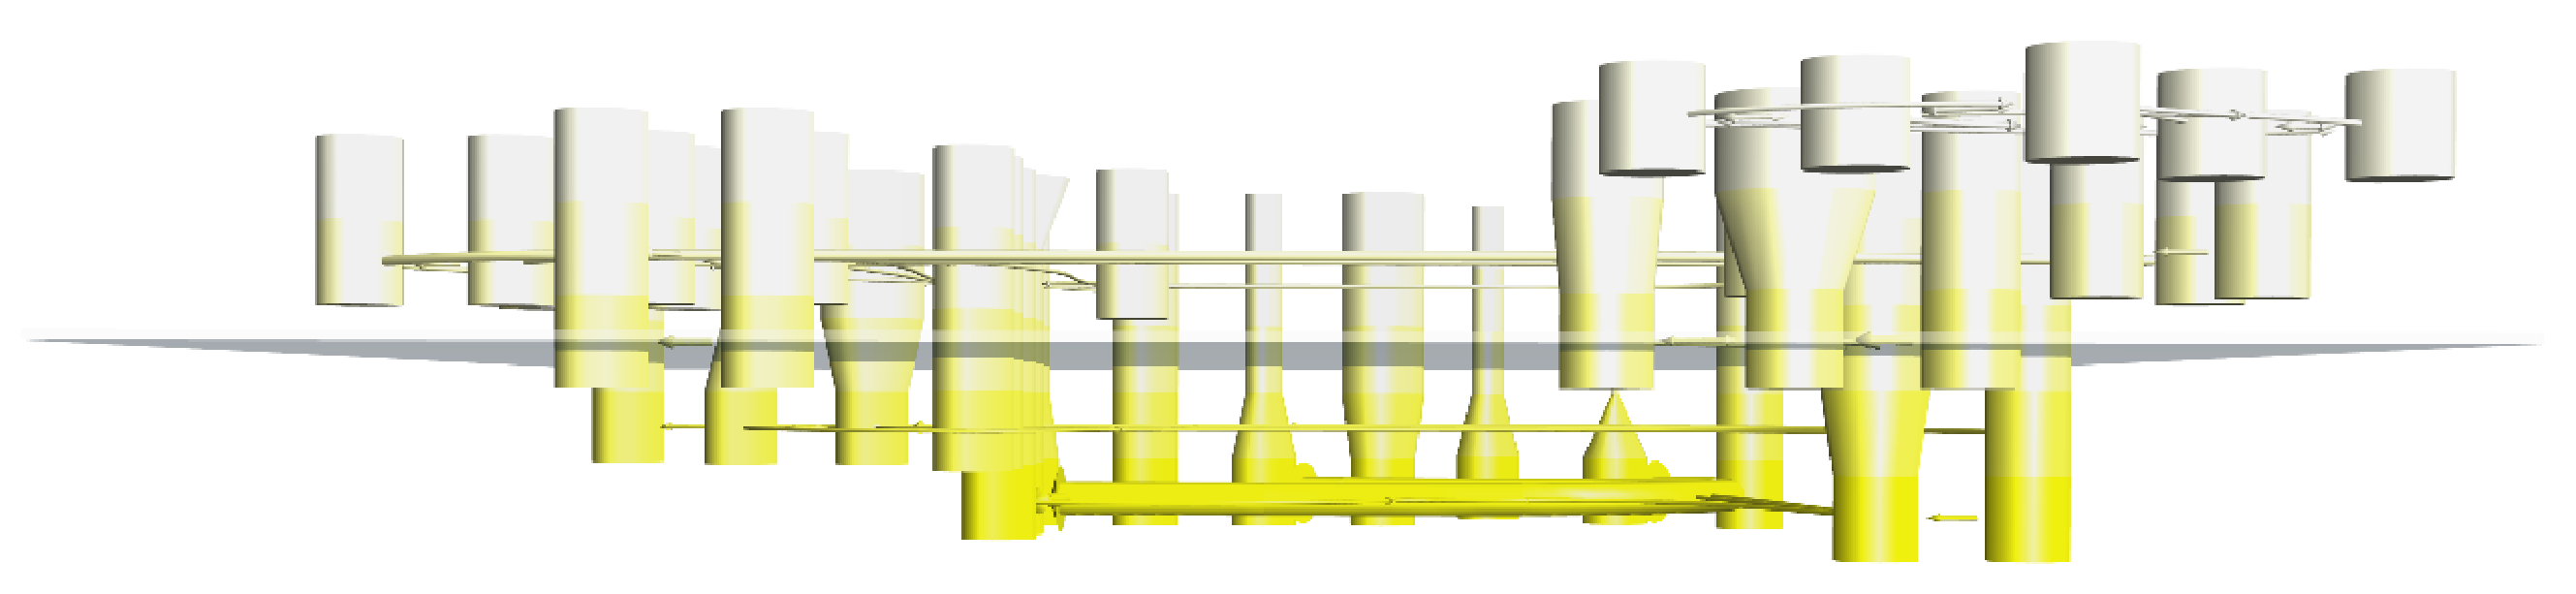
\includegraphics[width=0.4\textwidth]{figures/dot_waterlevel2_sideview.eps}}
  \caption{A visualisation of fund manager movement within the UK
  Computer Services sector for 5 time periods over 2 weeks in December.}
  \label{fig-fm}
\end{figure}

\subsubsection{Web Structure Visualisation}

One early application of Wilma was to the representation of web structure, and
to visualising clustering algorithms for categorising such
structure\cite{eckersley2kclassiscope}.

An example of web structure visualisation is shown in Figure~\ref{fig-web}.
This is a dataset collected in 2000 from the website \url{www.linuxlinks.com}.
The clusters are defined over similarity between pages; also note the set of
17 pages (linked to every other page) which form site's navigation bar.

\begin{figure}
\begin{center}
\scalebox{0.8}{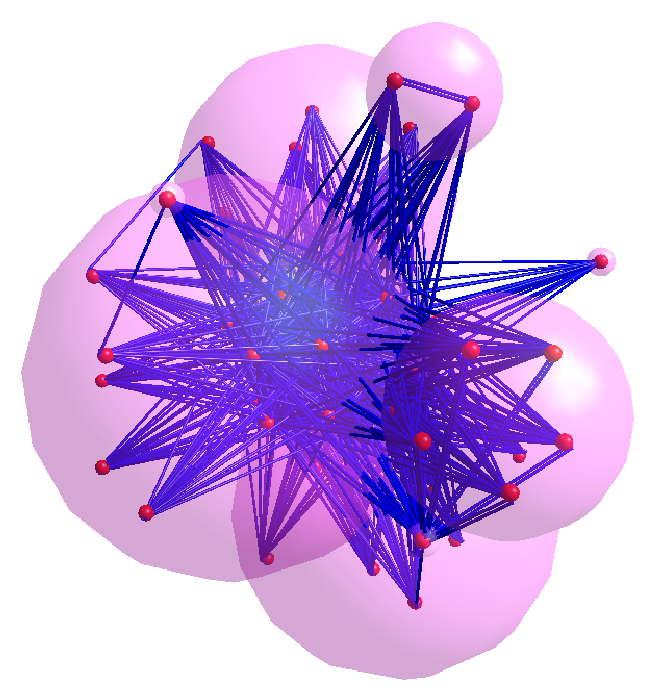
\includegraphics{figures/cluster1.eps}} \\
\caption{{\sc WilmaScope Visualisation of Web Site Structure}}
\label{fig-web}
\end{center}
\end{figure}

\begin{itemize}
\item pretty pictures
\item applications
\item self-congratulatory monologues
\end{itemize}

\section{Conclusions}
\label{sec:conclusions}

We hope that the reader will by now be convinced that WilmaScope presents an
invaluable addition to the graph connoisseur's toolbox.  

Wilma provides its users with animated, interactive 3D rendering, which takes
advantage of modern accelerated graphics hardware.  These facilities are, of
course, available by other means --- but Wilma's API and user interface
endeavours to provide them at a minimum of user labour and/or coding.

It has a general purpose, extensible architecture, enabling creative
experimentation, domain-dependent extensions, and successive layers of
functionality-transparency for users.

Finally, WilmaScope is released under a free software license --- the Lesser
GNU General Public License, or LGPL
(\url{http://www.gnu.org/copyleft/lesser.html}), which maximises benefits for
the user community, guarantees an open development ecology and thus encourage
creative hacking all round.

\paragraph{}

See you at \url{www.wilmascope.org}!

\begin{itemize}
\item megalomaniacal rants
\item further work
\item witty closing line
\end{itemize}

%\begin{thebibliography}{7}
%%
%\addcontentsline{toc}{section}{References}
%
%\bibitem{CHT93} Cai, J., Han, X., Tarjan, R.~E.\ (1993)
%An algorithm for the maximal planar subgraph
%problem.
%SIAM J.\ Comput.\ {\bf22}, 1142--1164
%
%\bibitem{DETT99} Di Battista, G., Eades, P., Tamassia, R., Tollis,
%  I.~G.\ (1999)
%Graph Drawing: Algorithms for the visualization of graphs.
%Prentice Hall, New Jersey
%
%\bibitem{Dji95} Djidjev, H.~N.\ (1995)
%A linear algorithm for the maximal planar subgraph problem.
%Proc.\ 4th Workshop Algorithms Data Struct., 
%Lecture Notes in Computer Science, Springer Verlag
%
%\bibitem{Eul1750} Euler, L.\ (1750)
%Demonstratio nonnullarum insignium proprietatum quibus solida hedris
%planis inclusa sunt praedita.
%Novi Comm.\ Acad.\ Sci.\ Imp.\ Petropol.\ {\bf4} (1752-3, published
%1758), 140--160, also: Opera Omnia (1) {\bf26}, 94--108
%
%\bibitem{KW01} Kaufmann, M., Wagner, D. (eds.) (2001)
%Drawing Graphs: Methods and Models.
%Lecture Notes in Computer Science 2025, Springer Verlag
%
%\bibitem{TDB88} Tamassia, R., Di Battista, G., Batini, C.\ (1988)
%Automatic graph drawing and readability of diagrams.
%IEEE Transactions on Systems, Man, and Cybernetics {\bf18}, 61--79
%
%\end{thebibliography}

\bibliographystyle{plain}
\newpage
\addcontentsline{toc}{section}{References}
\bibliography{refs}

%
%INDEX%%%%%%%%%%%%%%%%%%%%%%%%%%%%%%%%%%%%%%%%%%%%%%%%%%%%%%%%%%%%%%%
%\clearpage
%\addcontentsline{toc}{section}{Index}
%\flushbottom
%\printindex
%%%%%%%%%%%%%%%%%%%%%%%%%%%%%%%%%%%%%%%%%%%%%%%%%%%%%%%%%%%%%%%%%%%%%%

\end{document}
